\chapter{Überführung der Konzepte - Case Study \enquote{Tesla-Produktion}}
Ziel dieser Arbeit ist es, die Konzepte Operational \& Real-Time \ac{BI} anhand eines vereinfachten Beispiels zu veranschaulichen und Vor- und Nachteile abzuleiten. Hierzu wird eine hypothetische Case Study durchgeführt, in der eine Produktionsfirma simuliert wird. Aus den breiten Anwendungsmöglichkeiten der Konzepte wird sich für einen Produktionsbeispiel aufgrund der Annahme entschieden, dass dieses Beispiel für eine breite Menge an Personen leicht verständlich ist.
\section{Technische Umsetzung}
Um die Kontrolle über die Beispieldaten und damit die Nachvollziehbarkeit der Konzepte in der Praxis zu erhöhen, wurde davon abgesehen, eine bereits existierende \ac{DB} zu verwenden. Insbesodere die Aktualität der Daten im Sinne von Real-Time \ac{BI} macht eine solche Kontrolle erforderlich.
Aus diesem Grund wurde eine vollständige Konzeption der benötigten Informationen und Implementierung der Produktionslogik durchgeführt. Um das Verstädnis für die Ergebnisse dieser Arbeit zu erhöhen, werden die wichtigsten Aspekte der Technischen Umsetzung nachfolgend erläutert.
\subsection{Konzeptionierung}
\begin{figure}[]
    \centering
    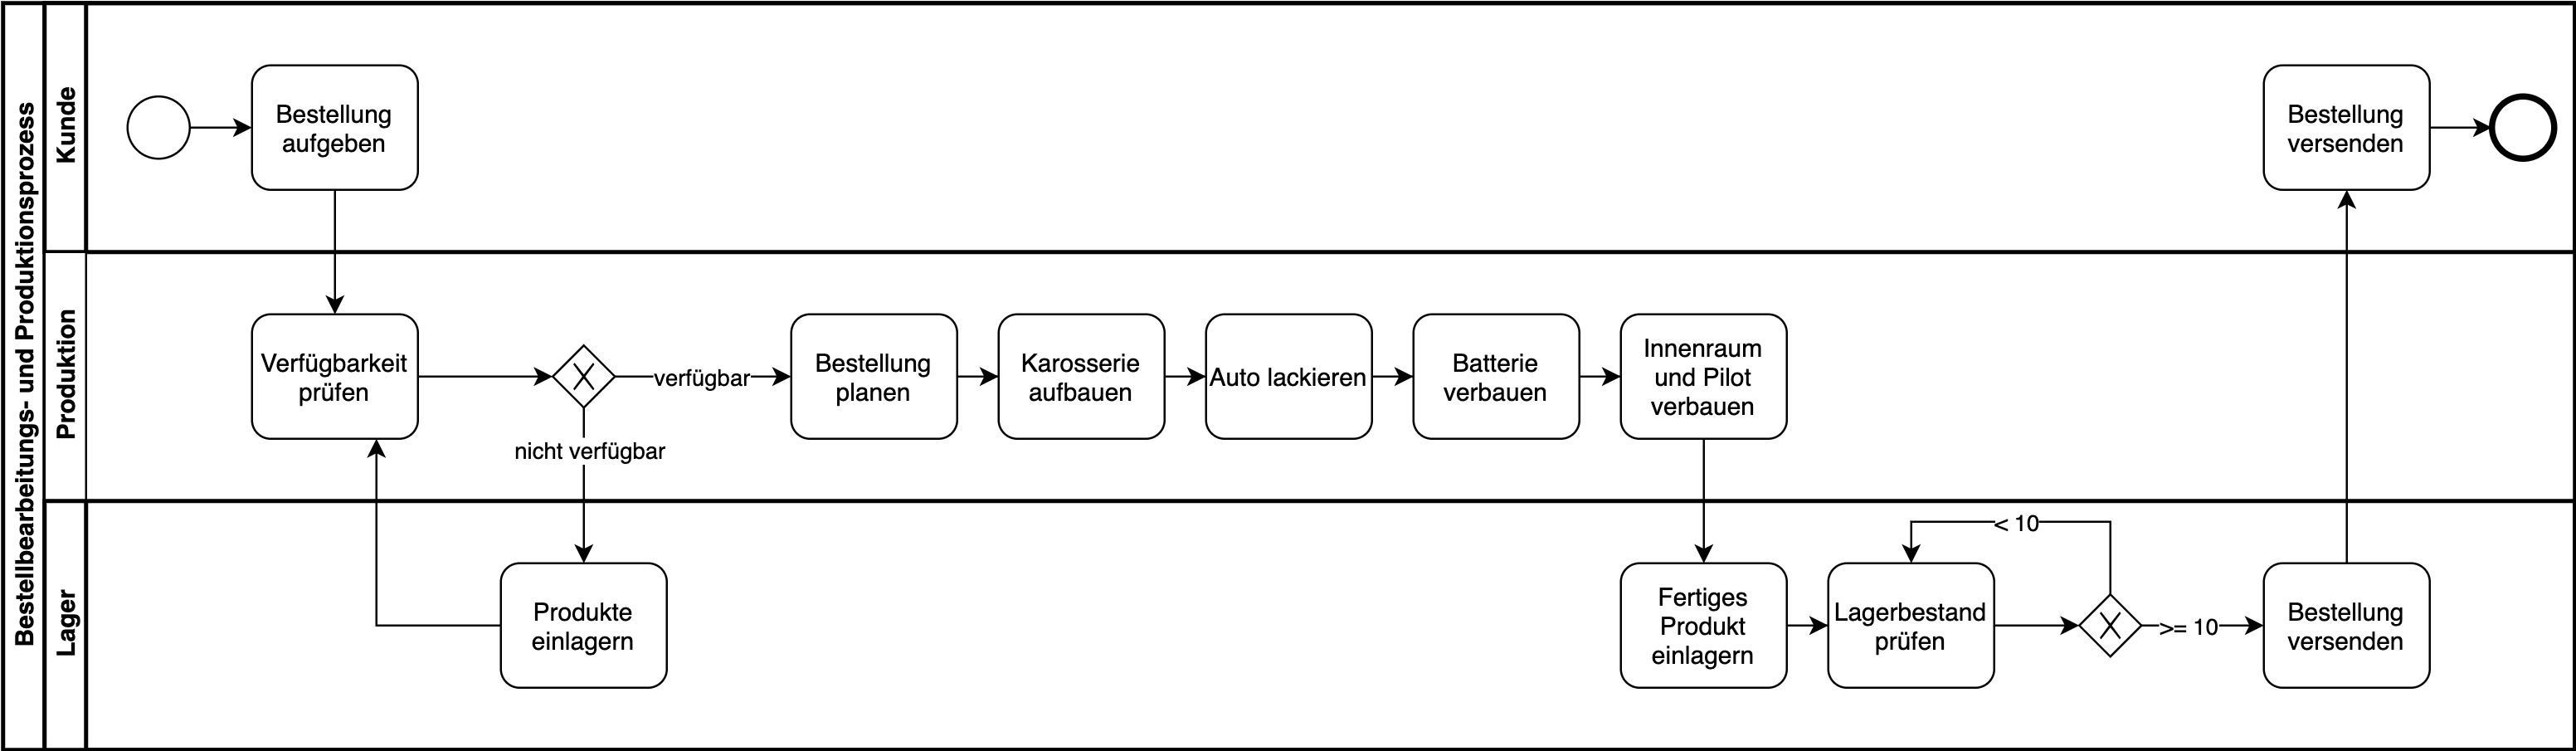
\includegraphics[width=\textwidth]{ausarbeitung-latex/img/Prozessmodell.png}
    \caption{Strategisches Prozessmodell}
    \label{fig:bpmn}
\end{figure}
Am Strategischen Prozessmodell (Abb. \ref{fig:bpmn}) wird der gewählte (reduzierte) Prozess für die Simulation deutlich. Nach dem Bestelleingang, wird die Bestellung geprüft, geplant und läuft anschließend durch den eigentlichen Produktionsprozess. Jedes Auto muss in der Produktion vier Stufen durchlaufen, wobei jede Stufe von einer Maschine durchgeführt wird:
\begin{enumerate}
    \item Karosserie: Hier wird das Grundgerüst des Autos aufgebaut. Es kann zwischen Model S, Model 3 und Model X gewählt werden.
    \item Farbe: In dieser Station wird das Auto entsprechend lackiert. Es kann zwischen Pearl White Multi-Coat, Solid Black, Midnight Silver Metallic, Deep Blue Metallic und Red Multi-Coat gewählt werden
    \item Batterie: Es gibt vier Batterien, die abhängig vom Typ verbaut werden können: Standard Plus, Maximale Reichweite, Performance, Plaid
    \item Innenraum und Pilot: Zuletzt wird der Innenraum (schwarz oder weiß) und Teile für die Steuerung (Autonomes Fahren oder Assistenz) verbaut.
\end{enumerate} 
Das fertige Produkt wird anschließend eingelagert und, sobald der Lagerbestand an fertigen Erzeugnissen über 10 steigt, versandt. Man kann sich vorstellen, dass es logistisch sinnvoll ist, den Versandprozess erst ab einer gewissen Menge an Produkte anzustoßen.

Für die technische Umsetzung wurde als Datengrundlage eine SQL-basierte, relationale \ac{DB} geschaffen (MariaDB). Diese gilt im Rahmen der Simulation als Single-Point-of-Truth und repräsentiert damit den Zustand der Produktionshalle. Damit kann die \ac{DB} als logische Repräsentation oder Digital Twin des hypothetischen, \ac{CPS} \textit{Fabrik} betrachtet werden
\begin{figure}[H]
    \centering
    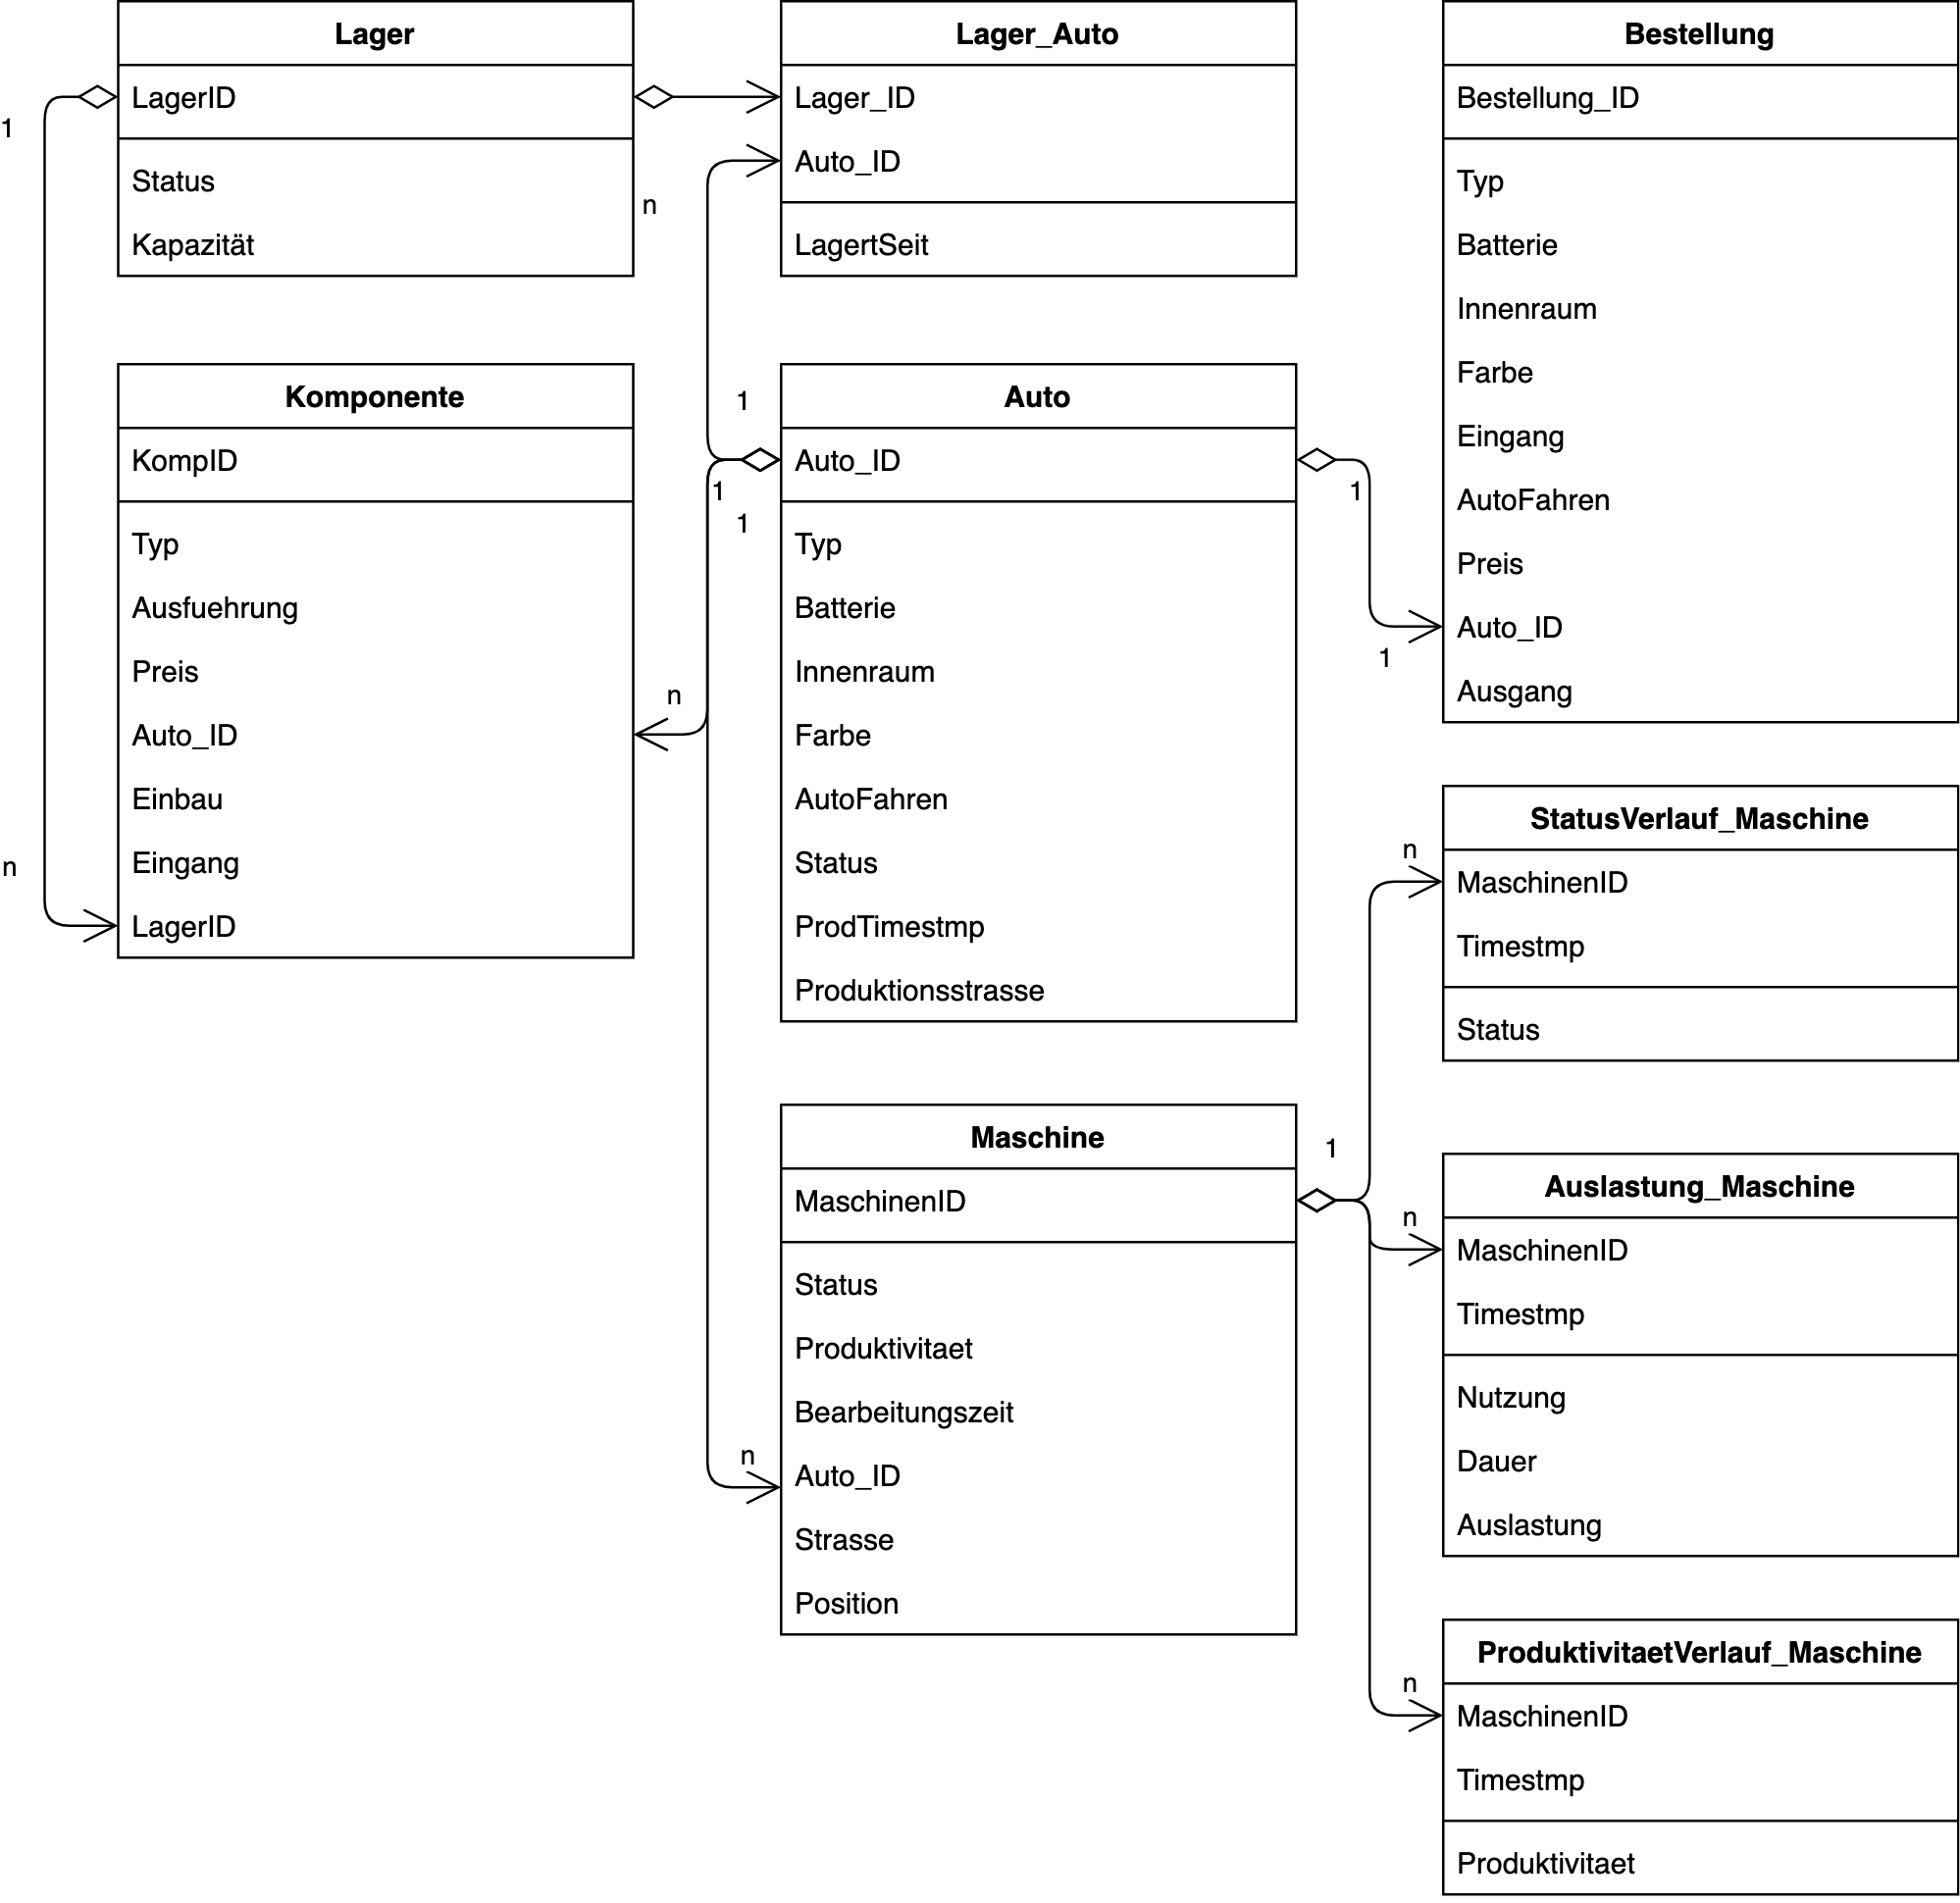
\includegraphics[width=0.7\textwidth]{ausarbeitung-latex/img/ER-Diagramm.png}
    \caption{ER-Diagramm}
    \label{fig:er}
\end{figure}
In Anbetracht des ER-Diagramms (Abb. \ref{fig:er}) wird der Bestellverarbeitungs- und Produktionsprozess (Abb. \ref{fig:bpmn}) ebenfalls deutlich: In Bestellung landen alle eingehenden Kundenbestellungen. Auf Basis dieser Bestellungen wird für jede Bestellung ein Auto generiert, dass der Konfiguration der Kundenbestellung entspricht. Diesem zu produzierendem Auto werden Komponenten zugeordnet. Es werden also nur Bestellungen geplant, deren Konfiguration in Form von Komponenten im Lager zu finden ist und damit produziert werden kann. Komponenten, die bereits einem Auto zugeordnet sind, werden hierfür nicht berücksichtigt.
\\Das entsprechende Auto befindet sich damit in der Produktionspipeline und erhält den Status 0 (geplant).
In einer Produktionsstraße gibt es vier Maschinen, wobei jede dieser Maschinen eine individuelle Grundbearbeitungszeit erhält. Dies ist die Zeit, die eine Maschine für das Einbauen des Teils in genau ein Auto bei einer Produktivität von 100\% benötigt. Innerhalb dieser Zeit werden die dem Auto zugeordneten Komponenten verbaut. Damit wird der individuelle Wert des Autos erhöht und die Komponente aus dem Lager entfernt. Das Auto durchläuft dabei Status 1 - 4. Nach Durchlaufen der letzten Maschine wird das Auto zunächst eingelagert (Status 5). Der Bestand an fertigen Erzeugnissen wird erst dann ausgeliefert, wenn 10 Bestellungen abgearbeitet wurden. Nach Lieferung ist das Auto befindet sich das Auto im finalen Status 6.
Eine Übersicht der verschiedenen Status einer Auto-Instanz findet sich in Tabelle \ref{tab:status}.
\begin{table}[H]
    \centering
    \begin{tabular}{|c|l|l|}
     \toprule
     \hline
         \textbf{Status}& \textbf{Beschreibung} & \textbf{Bedeutung} \\ \hline
          0 & geplant & Auto Instanz auf Basiss der Bestellung erzeugt und\\
           &&Komponenten zugeordnet\\
           &&Wert ist 0\\ \hline
          1 & Karosserie & Befindet sich in M1 oder wartet auf M2\\
          &&Wert nach Einbau entspricht Typ Komponente\\ \hline
          2 & Farbe & Befindet sich in M2 oder wartet auf M3\\
          &&Wert nach Einbau entspricht Wert in 1 zzgl. Preis \\
          &&Farbe\\ \hline
          3 & Batterie & Befindet sich in M3 oder wartet auf M4\\
          &&Wert nach Einbau entspricht Wert in 2 zzgl. Preis \\
          &&Batterie\\ \hline
          4 & Innenraum & Befindet sich in M4\\
          &und Pilot&Wert entspricht Wert in 3\\ \hline
          5 & lagernd& Befindet sich im Lager\\
          &&Wert entspricht Summe der Komponentenpreise\\ \hline
          6 & geliefert& Außerhalb des Prozesses\\ \hline
    \bottomrule
    \end{tabular}
    \caption{Status und Wert Auto Instanz}
    \label{tab:status}
\end{table}
Neben den Information, die notwendig sind, um den Bestellverarbeitungs- und Produktionsprozess abbilden zu können, werden weitere Informationen in der \ac{DB} gespeichert. Diese stellen Kennzahlen dar oder dienen der Berechnung dieser Kennzahlen im Sinne von Operational \& Real-Time \ac{BI}. Näheres zu den Kennzahlen findet sich in den Abschnitten \ref{abs:Kenn} und \ref{abs:anwOP}.

\subsection{Produktions-Simulation und Kennzahlenberechung} \label{abs:Kenn}
 Um Berichterstattung im Sinne von \ac{BI} zu ermöglichen wurde ein Simulationsskript geschaffen, das den Zustand der \ac{DB} in einem regelmäßigen Abstand erneuert\footnote{Der gesamte Code ist unter \url{https://github.com/leventlukas/digital-boardroom.git} aufrufbar.}. Dadurch wird der Produktionsprozess widergespiegelt. Zusätzlich wurden mehrere Web-UIs geschaffen, die eine direkte Manipulation der \ac{DB} ermöglichen. Konkret kann hierüber eine Bestellung getätigt, der Lagerbestand an Rohstoffen erhöht und Einfluss auf den Maschinen-Status genommen werden. Im Folgenden wird auf für den weiteren Verlauf dieser Arbeit relevante Zeilen eingegangen:

\textbf{Leistungsgrad}: Der Leistungsgrad ist definiert als der Quotient der Produktiven Zeit durch die gesamte Arbeitszeit. In jeder Iteration des Simulationsskriptes wird bestimmt, ob eine Maschine in der Zeit zur letzten Iteration gearbeitet hat. Hierfür wird geprüft, ob aktuell ein Auto in der Maschine ist. Wenn dies der Fall ist, wird Nutzung auf True gesetzt\footnote{simulation-backend/code/server.py,  Z. 212, 213}, andernfalls
 auf False\footnote{simulation-backend/code/server.py, Z. 337}. Die Nutzung wird zum aktuellen Zeitpunkt mit der Dauer in Auslastung\_Maschine gespeichert. Zusätzlich wird der Leistungsgrad über die letzten zehn Einträge gespeichert. Konkret wird der Quotient der Summe aller Einträge für Dauer, mit Nutzung True, und der Summe aller Einträge für Dauer gesamt berechnet und eingetragen\footnote{simulation-backend/code/server.py, Z. 321-333, 343, 433-438}. Damit stellt Spalte Auslastung der Tabelle Auslastung\_Maschine den gleitenden Durchschnitt des Leistungsgrades im zeitlichen Verlauf je Maschine dar.
 \begin{equation}\label{equ:nutz}
    Leistungsgrad_t = \frac{\sum_{i=t-10}^{t-1} Nutzungsdauer_i}{\sum_{i=t-10}^{t-1} Laufzeit_i}
\end{equation}

\textbf{Produktivität}: Die Produktivität beschreibt die prozentuale Leistungsfähigkeit einer Maschine in Relation zu ihrer Maximalen Leistungsfähigkeit und bestimmt damit die Bearbeitungszeit der Maschine. Sie kann direkt über das Web-UI \textit{Maschinenmanipulation} beeinflusst werden. Das Verhältnis von tatsächlicher Bearbeitungszeit und idealer Bearbeitungszeit in Abhängigkeit von der Produktivität kann durch Gleichung \ref{equ:prod} beschrieben werden. Die tatsächliche Bearbeitungszeit dient der Bestimmung, ob eine Maschine die Bearbeitung des Autos abgeschlossen hat\footnote{simulation-backend/code/server.py, Z. 196, 618-629, 214-218}. Über diesen Zusammenhang beeinflusst die Produktivität den Leistungsgrad der Maschine.
\begin{equation}\label{equ:prod}
    t_{tatsächlich} = t_{ideal}*(p*0.01)^{-1}
\end{equation}

\textbf{Komponentenpreis}: Der Preis einer Komponente entspricht dem Einkaufspreis und definiert in Summe den Wert eines bestimmten Autos. Umgekehrt ist der Wert eines Autos durch die Summe der Preise der verbauten Komponenten definiert. Neue Komponenten können direkt über das Web-UI \textit{Bestellung} mit manipulierten Preisen in das Lager überführt werden. Hierüber wird indirekt Einfluss auf die Materialkosten der zu produzierenden Autos genommen \footnote{simulation-backend/code/server.py, Z. 232-281}.

\textbf{Marge}: Die Marge der aktuellen Produktionspipeline ist definiert als die Summe der Umsätze einer Bestellung in der Produktionspipeline abzüglich der Herstellungskosten der Autos (Deckungsbeitrag 1) durch den Umsatz. Als Produktionspipeline sind alle Autos definiert, deren Status kleiner 5 ist, also noch nicht eingelagert sind. Die Herstellungskosten setzen sich zusammen als die Summe der Komponentenpreise. Dieser Zusammenhang ist in den Gleichungen \ref{equ:HK} und \ref{equ:Ma} dargestellt. Hierüber beeinflusst der Preis der Komponenten die Marge. Die Simulation geht von einer \ac{LiFo}-Systematik aus. Das bedeutet, dass die neusten Komponenten für die Planung aktueller Bestellungen verwendet werden \footnote{simulation-backend/code/server.py, Z. 400-441}. Die Berechnung erfolgt direkt über Abfrage von der \ac{DB} (Quelltext \ref{code:MSQL}).
\begin{equation}\label{equ:HK}
    Herstellungskosten_{Bestellung} = \sum Komponentenpreis_{Auto}
\end{equation}
\begin{equation}\label{equ:Ma}
    Marge_{Gesamt} = \frac{\sum Umsatz_{Bestellung} - \sum Herstellungskosten_{Bestellung}}{\sum Umsatz_{Bestellung}}
\end{equation}
\begin{lstlisting}[language=SQL, caption=Margenberechnung (SQL), label=code:MSQL]
SELECT Bestellung.Typ, m1.Status, m1.Typ, 
SUM(m1.Materialkosten) AS Materialkosten, 
SUM(Bestellung.Preis) AS Umsatz, 
((SUM(Bestellung.Preis) - SUM(m1.Materialkosten)) / SUM(Bestellung.Preis)) AS MargeSM
FROM Bestellung 
NATURAL JOIN (
    SELECT Auto.Auto_ID, Auto.Status, AS VerbauterWert,
    SUM(Komponente.Preis) AS Materialkosten 
	FROM Auto JOIN Komponente ON Auto.Auto_ID = Komponente.Auto_ID 
	GROUP BY Auto.Auto_ID
) AS m1
WHERE m1.Status <=4
GROUP BY Bestellung.Typ
\end{lstlisting}

\subsection{Architekturübersicht}
Die Übertragung der Konzepte Operational \& Real-Time-\ac{BI} in die vorgestellte Case Study lebt von dem Zusammenspiel der folgenden Komponenten: 
\begin{enumerate}
    \item Das Simulationsskript dient dazu, in regelmäßigen Abständen den Zustand der \ac{DB} zu aktualisieren. Es werden externe Veränderungen in der \ac{DB} berücksichtigt und in einen konsistenten Zustand überführt. Hierbei wird auf den vorherigen Zustand zugegriffen und die Veränderung auf Basis der verstrichenen Zeit abgeleitet und zurück in die \ac{DB} geschrieben.
    \item Über Konfigurator und Simulator kann direkter Einfluss auf die \ac{DB} genommen werden: Es können Bestellungen getätigt, Maschinenproduktivität beeinflusst und der Lagerbestand zum aktuellen Marktpreis der Komponenten erhöht werden.
    \item Dieser Zustand ist dann Anhand des Dashboards einsehbar. Eine genaue Erläuterung der Daschboards und der Grafiken in Bezug auf ihre unternehmerische Bedeutung erfolgt in Abschnitt \ref{abs:anwOP}.
\end{enumerate}
\begin{figure}[h]
    \centering
    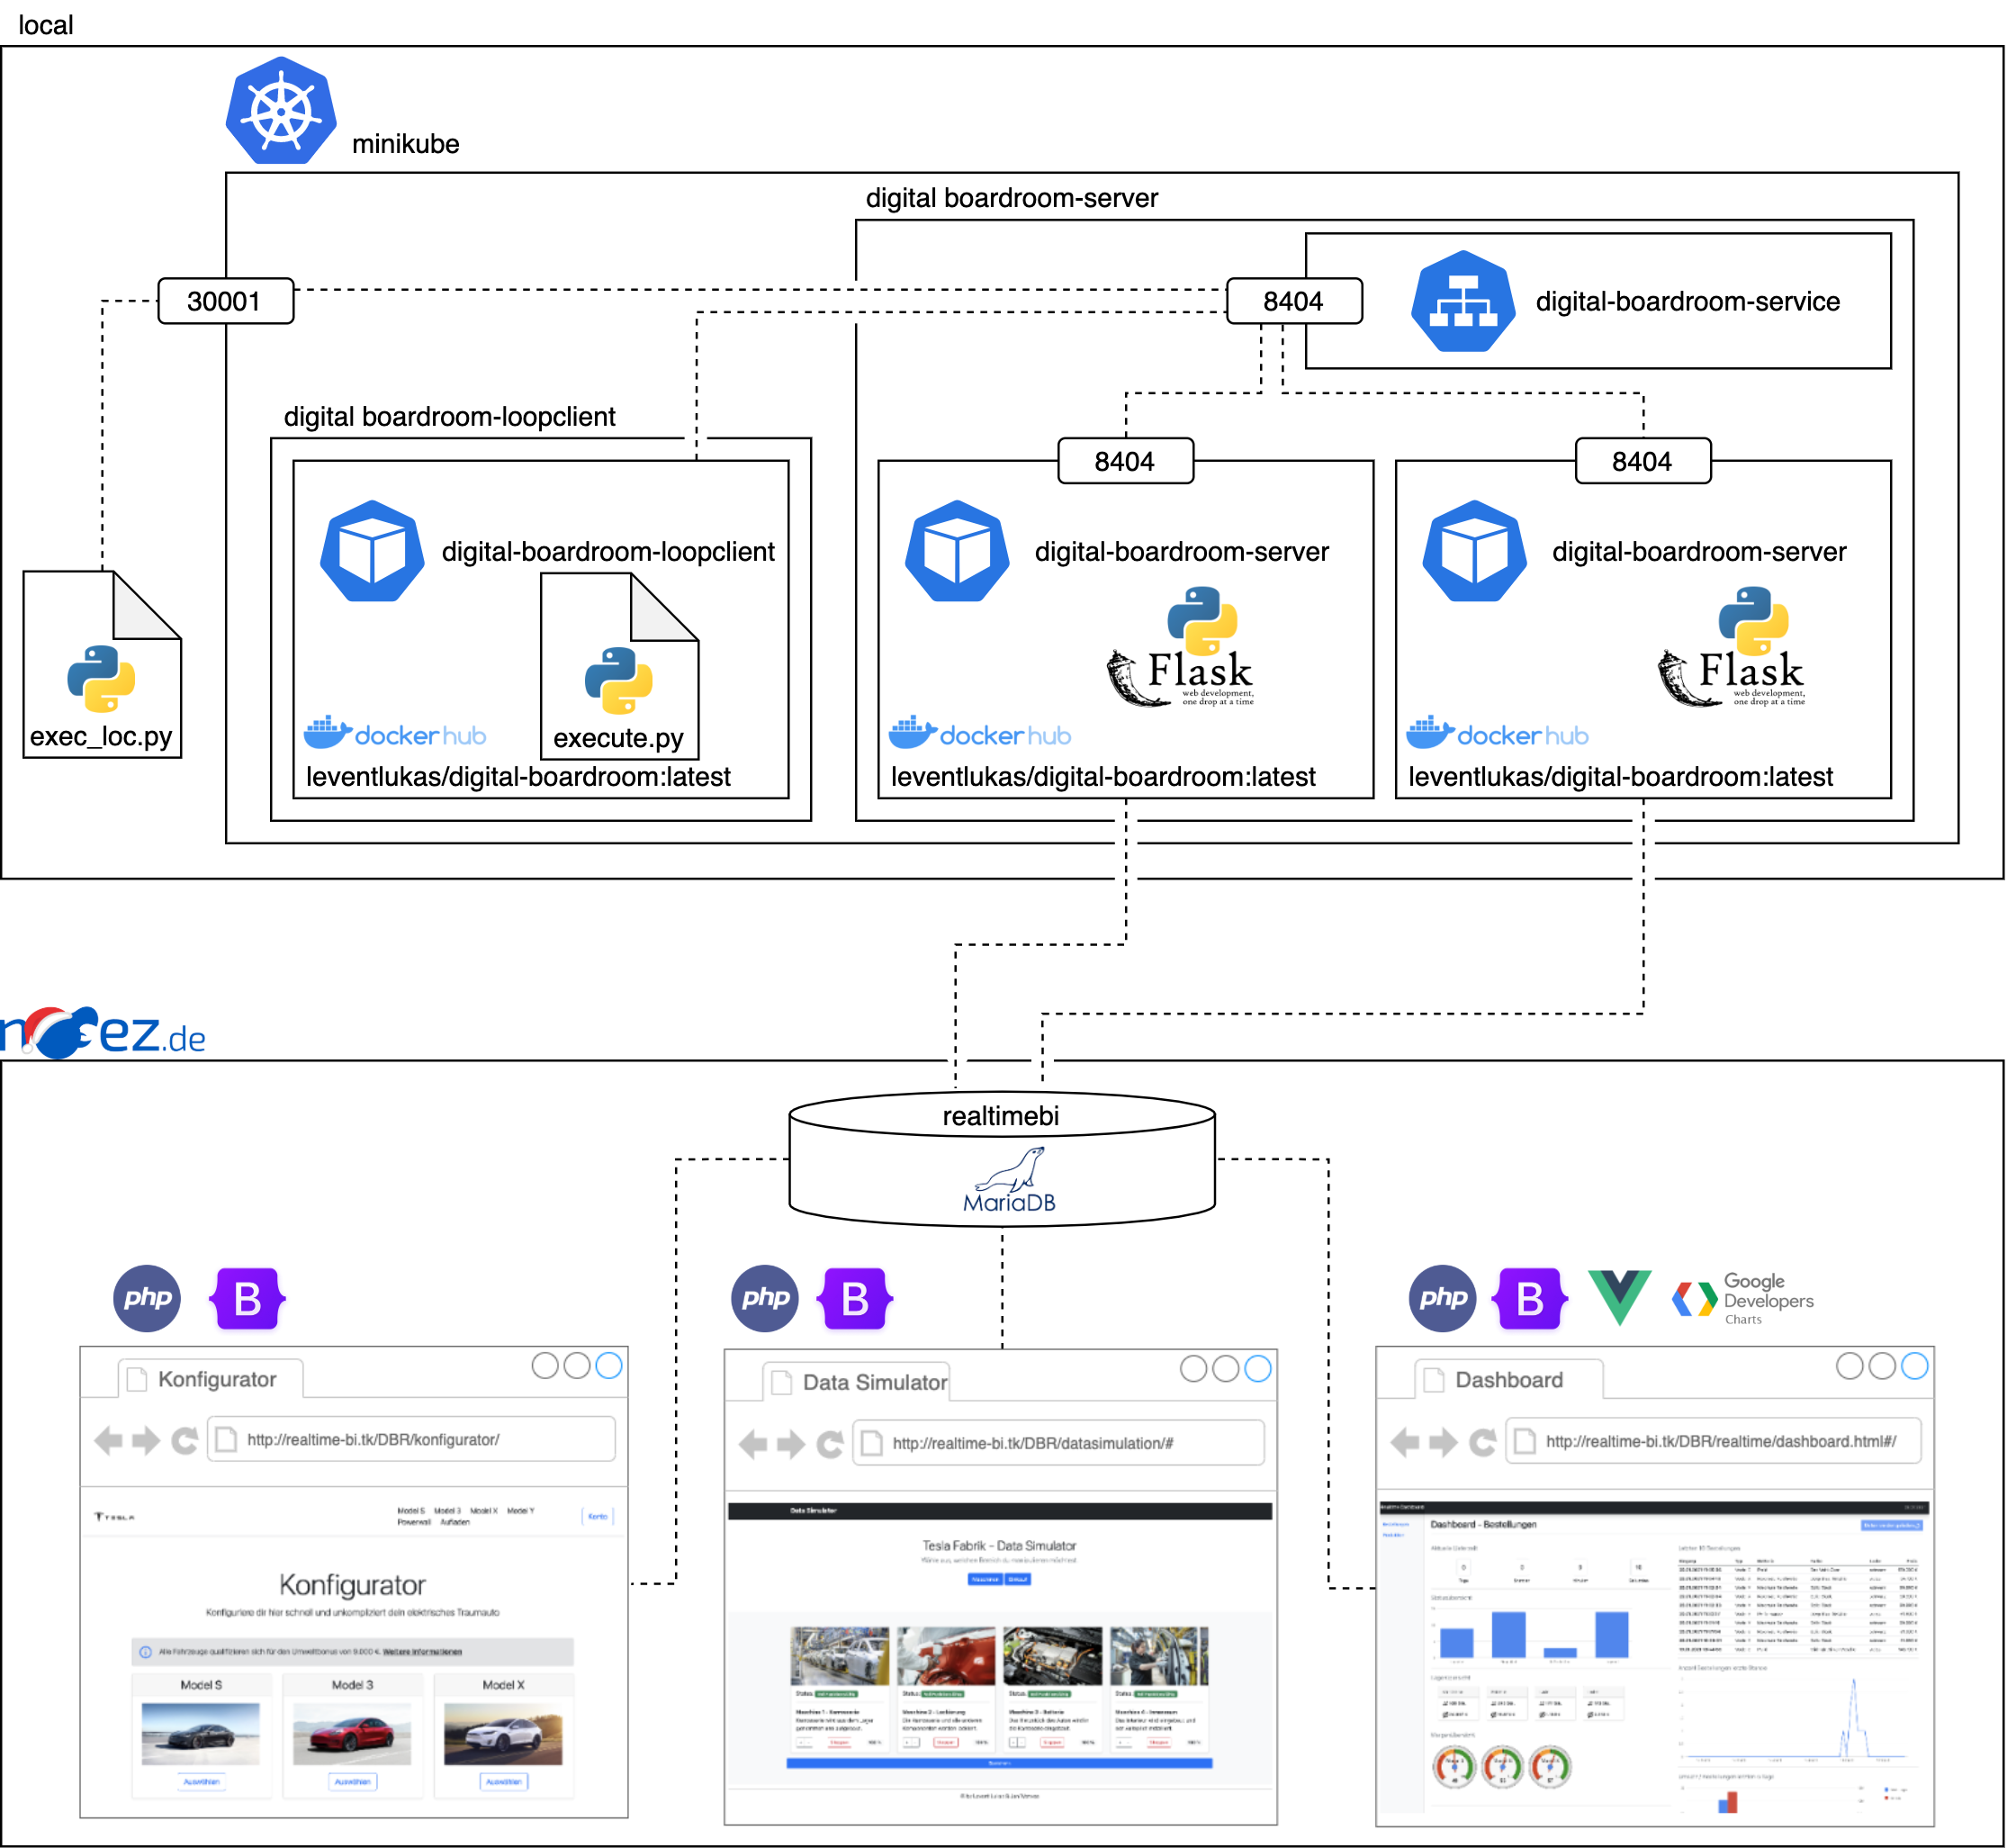
\includegraphics[width=0.99\textwidth]{ausarbeitung-latex/img/Architektur-Vertikal.png}
    \caption{Architektur}
    \label{fig:arch}
\end{figure}
Technisch wurde sich bei der Simulationskomponente für eine Microservice-Architektur, die auf einem lokalen Kubernetes-Cluster läuft, entschieden. Es gibt zwei Deployments: Das \textit{digitalboardroom-server} Deployment startet den Simulations-Server, der das Simulationsskript als Service bereitstellt. Diese Ressource ist repliziert und wird über einen NodePort-Service verfügbar gemacht. Der Service fungiert zusätzlich als LoadBalancer. Dieser Service wird vom \textit{digitalboardroom-loopclient} im gleichnamigen Deployment in einer Schleife alle 3 Sekunden konsumiert. Zusätzlich besteht die Möglichkeit, den Service außerhalb des Clusters lokal zu adressieren. Alle Pods basieren auf dem gleichen Dockerimage, besitzen jedoch unterschiedliche Entrypoints. Image-Versionen werden über Dockerhub verwaltet. Die Server-Replikas haben direkten Zugriff auf die \ac{DB}.
Die \ac{DB}, sowie die Web-UI's werden über noez.de gehostet. Die beiden Web-UI's zur direkten Manipulation sind über php und bootstrap umgesetzt. Für die Dashboards wurde zusätzliche vue.js \footnote{\url{https://vuejs.org}} und Google Developers Charts \footnote{\url{https://developers.google.com/chart}} verwendet. Die gesamte Architektur ist in Abb. \ref{fig:arch} dargestellt.

Für die verwendeten Tools wurde sich in dieser Ausarbeitung entschieden, da sie die für Real-Time \ac{BI} nötigen Funktionen im vollen Umfang kostenfrei zur Verfügung stellen. Insbesondere sind hiermit Datensynchronisation und Kollaboration gemeint. Andere Tools wie beispielsweise Microsoft Power BI bieten diesen Funktionsumfang ausschließlich in der kostenpflichtingen, professionellen Version.

\section{Anwendung Operational \& Real-Time BI} \label{abs:anwOP}
Die Anwendung der Konzepte\footnote{Eine Video-Demo kann unter folgenden Link abgerufen werden: \url{https://youtu.be/xnNvUQCp5Rk}} lässt sich in zwei Bereiche unterscheiden:
\begin{itemize}
    \item \textbf{Dashboard Bestellungen} (Abb. \ref{fig:DashBest}): Hierbei handelt es sich um eine Echtzeit-Übersicht der Bestellungen und verbundenen Kennzahlen. Damit stellt dieses Dashboard eine betriebswirtschaftliche Perspektive auf den aktuellen und zukünftigen Produktionsstatus dar. Es können beispielsweise Einkaufs- und Preisbildungsentscheidungen getroffen werden.
    \item \textbf{Dashboard Produktion} (Abb. \ref{fig:DashProd}): Hierbei handelt es sich um eine operative Sicht auf die Produktion. Es wird der aktuelle Status der Produktionshalle dargestellt, um operative Entscheidungen in Hinblick auf Maschinen und Produktion abzuleiten.
\end{itemize}
Im Folgenden werden die Elemente der Dashboards erläutert und Implikationen für operative Enscheidungen abgeleitet.
\subsubsection*{Dashboard Bestellung}
\begin{figure}[h]
    \centering
    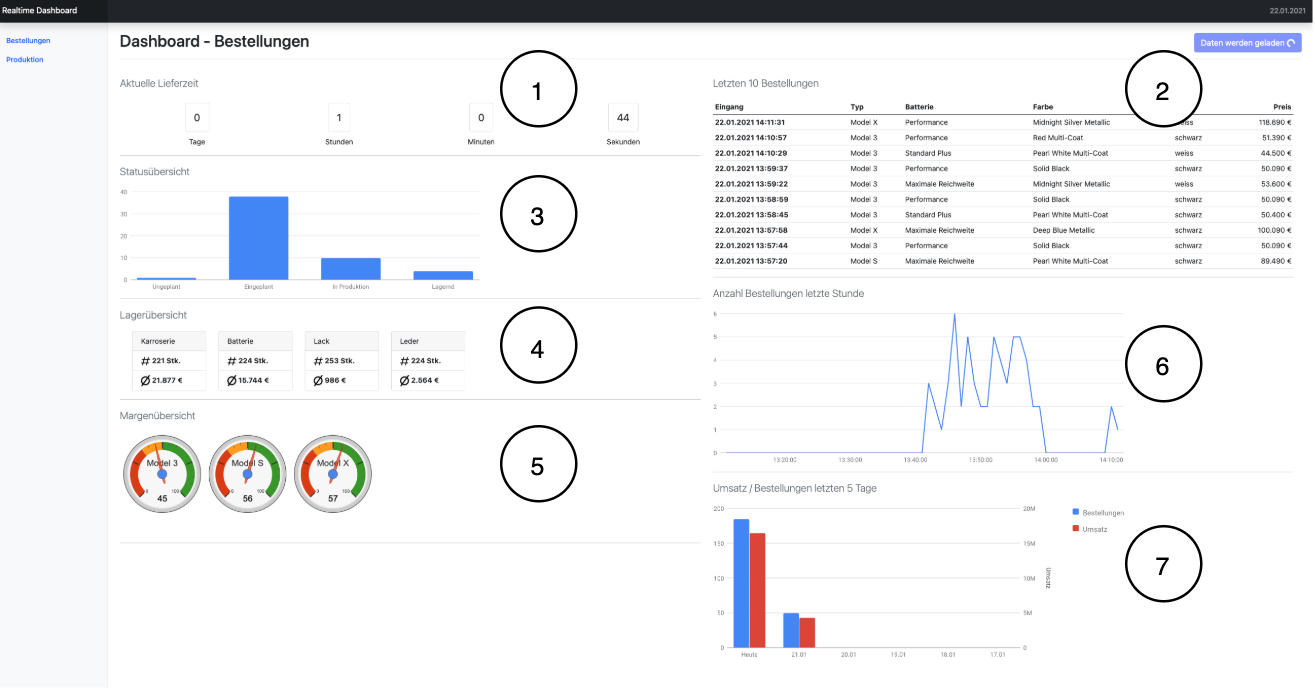
\includegraphics[width=1\textwidth]{ausarbeitung-latex/img/DashboardBestellung.png}
    \caption{Dashboard Bestellung}
    \label{fig:DashBest}
\end{figure}
\begin{enumerate}
    \item Aktuelle Lieferzeit: Die aktuelle Lieferzeit ist definiert als die Differenz der Zeitpunkte Bestellungseingang und Versand der Bestellungen. Da das Lager ab zehn fertigen Produkten geleert und die Produkte versendet werden, werden hier die letzten zehn Bestellungen betrachtet. Sinkende Kundenzufriedenheit kann Folge einer erhöhten Lieferzeit sein. Gründe können unzureichender Lagerbestand oder Probleme in der Porduktion sein. Diese können anhand der Graphiken drei und vier abgeleitet werden.
    \item Letzten 10 Bestellungen: Die letzten zehn Bestellungen geben Auskunft über die Entwicklung der Kundenbedürfnisse. Es können Entscheidungen für den Einkauf abgeleitet werden.
    \item Statusübersicht: Diese Pipeline gibt eine Übersicht darüber in welchem Schritt sich die Bestellungen aktuell befinden. Fehlt es beispielsweise an den richtigen Komponenten, um die aktuellen Kundenbedürfnisse zu befriedigen, erhöht sich der Anteil der ungeplanten Bestellungen; Kommt es dagegen zu Problemen in der Produktion, erhöht sich der Anteil an geplanten Bestellungen oder in Produktion.
    \item Lagerübersicht: Die Lagerübersicht gibt Aufschluss über den Anteil und den durchschnittlichen Preis der Komponenten im Lager. Damit können Entscheidungen für den Einkauf getroffen werden. Wenn sich der Lagerbestand zu sehr verringert, steigt die Wahrscheinlichkeit, dass die Konfiguration bestimmter Bestellungen nicht befriedigt werden kann; Gleichzeitig stellen die durchschnittlichen Preise eine Referenz für den Einkauf dar, was insbesondere durch die Margenübersicht an Relevanz gewinnt.
    \item Margenübersicht: Die Margenübersicht setzt die Kosten in das Verhältnis zu den Umsätzen der Bestellungen, die sich in der Produktionspipeline befinden (Gl. 3.4). Da hier weitere Kosten hinzukommen, ist der inakzeptable Bereich recht hoch. Die Margen unterscheiden sich für jeden Typ und jede Konfiguration. Sinken die Verkaufspreise oder steigen die Einkaufspreise der Komponenten, wird dies direkt in der Margenübersicht deutlich und es können entsprechende Maßnahmen getroffen werden.
    \item Anzahl Bestellungen der letzten Stunde: Die Anzahl der Bestellungen zeigt deutlich Anomalien im Verhalten der Kunden. Drastische Ausschläge in die eine oder andere Richtung, können - je nach Richtung des Ausschlags - zu Lieferunfähigkeit oder fehlenden Deckungsbeiträgen führen.
    \item Umsatz/Bestellungen: Zuletzt bietet diese Übersicht eine Einordnung des Umsatzes und der Anzahl der Bestellungen im Verhältnis zu den letzten fünf Tagen. Eine systematische Veränderung dieser Zahlen können Maßnahmen erforderlich machen (z.B. Werbekampagne schalten/erhöhen).
\end{enumerate}

\subsubsection*{Dashboard Produktion}\label{abs:dashProd}
\begin{figure}[h]
    \centering
    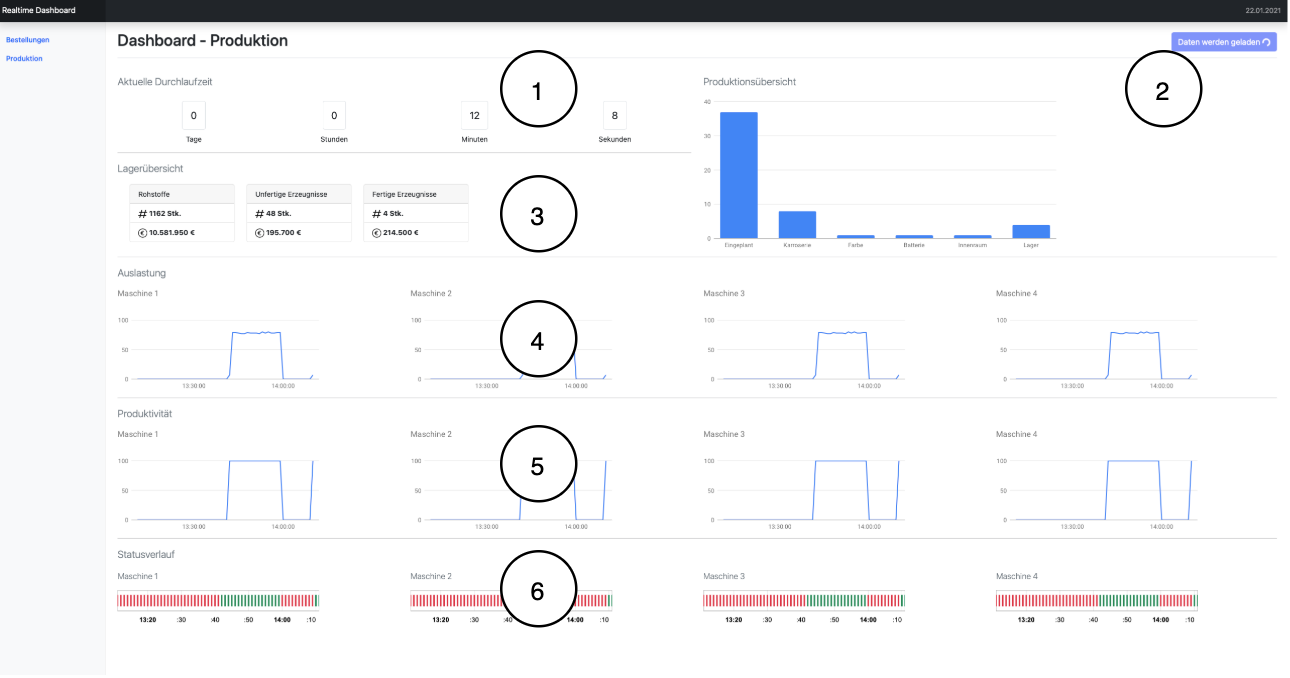
\includegraphics[width=1\textwidth]{ausarbeitung-latex/img/DashboardProduktion.png}
    \caption{Dashboard Produktion}
    \label{fig:DashProd}
\end{figure}
\begin{enumerate}
    \item Aktuelle Durchlaufzeit: Die aktuelle Durchlaufzeit ist eine der wichtigsten Kennzahlen der Produktion und dient als initialer Indikator. Nähere Informationen über die Gründe einer Erhöhung wird in den anderen Elementen des Dashboards deutlich.
    \item Produktionsübersicht: Die Produktionsübersicht gibt an, wie viele Autos sich in welcher produktionsbezogenen Station (Tab. \ref{tab:status}) befinden. Da die Produktion an einem One-Piece-Flow orientiert ist, ist die Erwartung, dass sich in jeder Station ein Auto befindet. Verringert sich die Produktivität einer Maschine, drückt sich dies in einem Stau an der vorherigen Station aus.
    \item Lagerübersicht: Die Lagerübersicht unterscheidet in Rohstoffe, fertige und unfertige Erzeugnisse. Eine Erhöhung der Durchlaufzeit hat eine Erhöhung des Lagerbestandes an unfertigen Erzeugnissen zur Folge, was negative bilanzielle Implikationen hat.
    \item Maschinenauslastung: Die Maschinenauslastung entspricht dem Verlauf des Leistungsgrades (Gl. 3.1). Die Abnahme der Maschinenauslastung ist auf eine verringerte Produktivität der Vormaschine zurückzuführen. Diese Maschine weist dann einen gestiegenen Leistungsgrad auf, da sich durch die erhöhte Bearbeitungszeit, ein Produktstau an der Station vor dieser Station bildet. Dies wird ebenfalls in der Produktionsübersicht deutlich.
    \item Maschinenproduktivität: Die Produktivität gibt Aufschluss auf die tatsächliche Bearbeitungszeit (Gl. 3.2) und kann somit als Erklärung der anderen Kennzahlen herangezogen werden.
    \item Maschinenstatusverlauf: Zuletzt bietet der Statusverlauf sofortige Auskunft über den Zustand einer Maschine und dient ebenfalls der Erlärung anderer Kennzahlen. Zusammen mit den bereits vorgestellten Kennzahlen können Entscheidungen über Wartung und Konfiguration einzelner Maschinen bzw. der Produktion getroffen werden.
\end{enumerate}
\section{Ergebnisse}
Anhand der Überführung der Konzepte Operational \& Real-Time \ac{BI} werden diese nicht nur verständlich, sondern die Vor- und Nachteile werden greifbar: Auf der einen Seite erlaubt die implementierte Lösung die Überwachung und Steuerung der zugrundeliegenden Prozesse. Hierdurch können Probleme in der Produktion schnell erkannt und gelöst werden. Dies bildet die Grundlage für eine Prozessverbesserung. Dadurch und durch den Einblick in die Kostenstruktur ergibt sich die Möglichkeit zur Kosteneinsparung, was einen Wettbewerbsvorteil bewirkt. Von der Implementierung einer Decision-Engine wurde im Rahmen dieses Projektes abgesehen, da dies die Interaktivität der Lösung beeinflussen und somit die Verständlichkeit reduzieren würde. Zumal im Rahmen der Simulation zur Verdeutlichung mit Bearbeitungszeiten von einigen Sekunden gerechnet wird. Da es sich bei dem gewählten Konzept um eine Web-basierte Lösung handelt, ist diese auch prinzipiell allen möglichen Mitarbeiter verfügbar. 
\\Auf der anderen Seite wird die Kostenintensität einer \ac{BI}-Lösung anhand der Komplexität des umgesetzten Beispiels deutlich. Die Tatsache, dass es sich bei der vorliegenden Implementierung um ein reduziertes Beispiel handelt, unterstreicht diesen Aspekt zusätzlich.

Weitere Ergebnisse dieser Arbeit ergeben sich in Bezug auf die verwendeten Technologien: Es wurde sich für eine Relationale \ac{DB} entschieden, was zu gelegentlichen Performanceproblemen führte. In der Praxis ist jedoch von der teilweisen Verwendung von Zeitreihendatenbanken\footnote{Bspw. Prometheus \url{https://prometheus.io}} auszugehen, die für die Verwendung von zeitbasierten Daten optimiert und sich damit für Real-Time \ac{BI} besonders eignen.
\\Auch für das Reporting sind andere Tools für den produktiven Einsatz besser geeignet, erhöhen jedoch Kosten und Komplexität. Zu nennen sind hier Microsoft Power BI oder Grafana\footnote{\url{https://grafana.com/grafana/}}.